%%%% 補助スライド
\appendix
\backupbegin

\begin{frame}{~}
 \centering
 - 補足用 -
\end{frame} 

%%%%%%%%%%%%%%%%%%%%%%%%%%%%%%%%%%%%%%%%%%%%%%%%%%%%%%%%%%%%%%%%%%%
\begin{frame}\frametitle{基本ソルバーの問題点}

  \begin{block}{}
    \centering
    $
    \varphi_{\ell-1} = S(\bm{x}^0)
    \land \bigwedge_{t=0}^{\ell-1} C(\bm{x}^t) 
    \land \bigwedge_{t=1}^{\ell-1} T(\bm{x}^{t-1},\bm{x}^{t})
    \land G(\bm{x}^{\ell-1})
    $
    $
      \varphi_{\ell} = S(\bm{x}^0)
      \land \bigwedge_{t=0}^{\ell} C(\bm{x}^t) 
      \land \bigwedge_{t=1}^{\ell} T(\bm{x}^{t-1},\bm{x}^{t})
      \land G(\bm{x}^\ell)
    $
  \end{block}
  
  
  \begin{itemize}
    \item $\varphi_{\ell-1}$と$\varphi_{\ell}$に含まれる制約のほとんどは同じである.
  \end{itemize}
  \begin{exampleblock}{}
    \centering
      \scalebox{0.8}{\begin{tabular}{r|ll|r}
  基となる論理式 & 追加する論理式 & 削除する論理式 & 生成される論理式 \\ \hline
  $\varphi_{\ell-1}$ & $C(\bm{x}^{\ell}), T(\bm{x}^{\ell-1},\bm{x}^{\ell}), G(\bm{x}^\ell)$ 
    & $G(\bm{x}^{\ell-1})$ & $\varphi_{\ell}$ \\
    $\varphi_{\ell}$ & $C(\bm{x}^{\ell+1}), T(\bm{x}^{\ell},\bm{x}^{\ell+1}), G(\bm{x}^{\ell+1})$ 
    & $G(\bm{x}^{\ell})$ & $\varphi_{\ell+1}$ \\ 
\end{tabular}}
  \end{exampleblock}

  %\begin{block}{$\varphi_{\ell-1}$と$\varphi_{\ell}$の共通要素と非共通要素}
  %  \centering
  %  $
  %    \varphi_{\ell -1} \land \varphi_{\ell} =
  %    \{S(\bm{x}^0) \land \bigwedge_{t=0}^{\ell-1} C(\bm{x}^t)
  %    \land \bigwedge_{t=1}^{\ell-1} T(\bm{x}^{t-1},\bm{x}^{t})\}
  %  $
  %  $
  %    \varphi_{\ell -1} \oplus \varphi_{\ell} = 
  %    \{C(\bm{x}^{\ell}), T(\bm{x}^{\ell -1}, 
  %    \bm{x}^{\ell}), G(\bm{x}^{\ell -1}), G(\bm{x}^{\ell})\}
  %  $
  %\end{block}
  \bigskip

  基本ソルバーでは各$\varphi_{\ell}$に対して,
  毎回 ASP システムを起動し実行するため,
  \begin{itemize}
    \item 学習節が引き継がれず同一の探索空間を繰り返し調べる必要がある.
    \item 同一のルールを繰り返し基礎化する必要がある.
  \end{itemize}
  といった問題点が存在する.

\end{frame}
%%%%%%%%%%%%%%%%%%%%%%%%%%%%%%%%%%%%%%%%%%%%%%%%%%%%%%%%%%%%%%%%%%%
\begin{frame}
  \frametitle{改良アルゴリズム}

  \begin{block}{改良アルゴリズムの手続き}
    \begin{enumerate}
      \item ファクト形式の問題インスタンスと,
            各制約に対応したルールを表す複数のサブプログラムから構成された
            論理プログラムを与える.
      \item ステップ数$t=0$とする.
      \item $t>0$であれば,ゴール状態の制約$G(\bm{x}^{t -1})$を
            表すルールを削除する. \label{improved_solver:loop}
      \item $t=0$であれば,スタート状態の制約$S(\bm{x}^0)$を
            表すルールを追加する.
      \item グラフ点彩色問題の制約$C(\bm{x}^{t})$と遷移制約$T(\bm{x}^{t-1},\bm{x}^{t})$
            を表すルールを追加する.
      \item ゴール状態の制約$G(\bm{x}^{t})$を表すルールを追加する.
      \item $\varphi_{t}$の到達可能性を検査する.
      \item ASP システムの出力が充足可能であれば終了する.
            充足不能であれば$t$の値を1増加させ,
            \ref{improved_solver:loop}に戻り手続きを繰り返す.
            \begin{itemize}
              \item ただし,$t$がステップ長の上限値を超えたところで
                    繰り返しを停止できる.
            \end{itemize} \label{improved_solver:end}
    \end{enumerate}
  \end{block}
\end{frame}
%%%%%%%%%%%%%%%%%%%%%%%%%%%%%%%%%%%%%%%%%%%%%%%%%%%%%%%%%%%%%%%%%%%
\begin{frame}[shrink]
  \frametitle{$k$彩色遷移問題を解く\code{unchanged} 符号化 {\small(基本ソルバー用)}}

\begin{columns}[t]
\begin{column}{0.9\linewidth}
\begin{exampleblock}{\code{unchanged.lp}}
\lstinputlisting[frame=none,numbers=left,basicstyle=\ttfamily\scriptsize]{code/gcrp_cc_unchanged.lp} 
\end{exampleblock}    
\end{column}
\end{columns}

\begin{itemize}
  \item 9--10行目: 遷移制約$T(\bm{x}^{t-1},\bm{x}^{t})$の表し方が,
    \code{changed}符号化と異なる.
  \item アトム\code{unchanged(X,T)}は,ステップ\code{T-1}とステップ\code{T}の間
    で,頂点\code{X}の色が変化しなかったことを意味する.
  \item 10行目: 各ステップ\code{T}において,色が変化しない頂点はちょうど
    \code{N-1}個であることを表す.
    \begin{itemize}
      \item \code{N}はグラフの頂点数を表す.
    \end{itemize}
\end{itemize}

\end{frame}
%%%%%%%%%%%%%%%%%%%%%%%%%%%%%%%%%%%%%%%%%%%%%%%%%%%%%%%%%%%%%%%%%%%
\begin{frame}[shrink]
  \frametitle{$k$彩色遷移問題を解く\code{changed} 符号化 {\small(改良ソルバー用)}}

\begin{columns}[t]
\begin{column}{0.9\linewidth}
\begin{exampleblock}{\code{changed_inc.lp}}
\lstinputlisting[frame=none,numbers=left,basicstyle=\ttfamily\scriptsize]{code/gcrp_cc_changed_inc.lp} 
\end{exampleblock}    
\end{column}
\end{columns}

\begin{itemize}
  \item 複数のサブプログラムから構成される.
    \only<1>{
      \begin{itemize}
        \item \code{based}ブロックはスタート状態の制約$S(\bm{x}^0)$を含む.
      \end{itemize}
    }
    \only<2>{
      \begin{itemize}
        \item \code{step}ブロックはグラフ点彩色問題の制約$C(\bm{x}^{t})$,
          遷移制約$T(\bm{x}^{t-1},\bm{x}^{t})$を含む.
      \end{itemize}
    }
    \only<3>{
      \begin{itemize}
        \item \code{check}ブロックはゴール状態の制約$G(\bm{x}^{\ell})$を含む.
      \end{itemize}
    }
    \only<4>{
      \item その他の部分は\code{changed}符号化の自然な拡張である.
    }
\end{itemize}
\end{frame}
%%%%%%%%%%%%%%%%%%%%%%%%%%%%%%%%%%%%%%%%%%%%%%%%%%%%%%%%%%%%%%%%%%%
\begin{frame}[shrink]
  \frametitle{基となるグラフごとの解けた問題数}
  
  \begin{exampleblock}{}
    \centering
    \scalebox{0.8}{\begin{tabular}{l|rrr|rrr}
  グラフ名 & 平均次数 & 色数$k$ & 実行可能解の総数 & 到達可能 & 到達不能 & 判定不能 \\ \hline
  1-FullIns\_3 & 6.67 & 4 & 50,693,280 & 1 & 0 & \structure{9} \\ 
  le450\_5a & 25.40 & 5 & 3,840 & 0 & 10 & 0 \\ 
  le450\_5c & 43.57 & 5 & 120 & 0 & 10 & 0 \\ 
  le450\_5d & 43.36 & 5 & 960 & 0 & 10 & 0 \\ 
  myciel3 & 3.64 & 4 & 12,480 & 5 & 0 & \structure{5} \\ 
  myciel4 & 6.17 & 5 & 2,845,658,400 & 5 & 0 & \structure{5} \\ 
  queen5\_5 & 12.80 & 5 & 240 & 0 & 10 & 0 \\  
  queen6\_6 & 16.11 & 7 & 100,800 & 0 & 10 & 0 \\ 
  queen7\_7 & 19.43 & 7 & 20,160 & 0 & 10 & 0 \\
\end{tabular}}
  \end{exampleblock}
  \begin{itemize}
    \item $\textrm{平均次数} = (\textrm{辺数}*2) / (\textrm{頂点数})$
    \item 色数$k$は彩色数に等しい.
    \item 難しい問題の特徴としては,基となる問題の実行可能解の総数が多いことや,
      平均次数と色数$k$の差が少ないことなどが考えられる.
      \begin{itemize}
        \item $k \ge \Delta(G) + 2$ならば到達可能である.
        \item $\Delta(G)$はグラフ$G$の最大次数である.
      \end{itemize}
  \end{itemize}
\end{frame}
%%%%%%%%%%%%%%%%%%%%%%%%%%%%%%%%%%%%%%%%%%%%%%%%%%%%%%%%%%%%%%%%%%%
\begin{frame}
  \frametitle{到達可能インスタンスのCPU時間による比較}

  \begin{exampleblock}{}
    \centering
    \scalebox{0.75}{\begin{tabular}{lr|rr|rr}
  \multicolumn{2}{r|}{} & \multicolumn{2}{c|}{基本ソルバー} & \multicolumn{2}{c}{改良ソルバー} \\
  問題名 & ステップ長 & \code{changed} & \code{unchanged} & \code{changed} & \code{unchanged} \\ \hline
  \code{1-FullIns_3_col4_1} & 11 & 1.374 & 1.071 & 1.291 & 0.756 \\
  \code{myciel3_col4_1} & 11 & 0.179 & 0.148 & 0.065 & 0.065 \\
  \code{myciel3_col4_3} & 11 & 0.206 & 0.164 & 0.082 & 0.080 \\
  \code{myciel3_col4_4} & 13 & 0.486 & 0.445 & 0.303 & 0.583 \\
  \code{myciel3_col4_7} & 8 & 0.090 & 0.072 & 0.042 & 0.036 \\
  \code{myciel3_col4_8} & 9 & 0.119 & 0.094 & 0.048 & 0.044 \\
  \code{myciel4_col5_2} & 16 & 42.482 & 48.721 & 20.308 & 134.056 \\
  \code{myciel4_col5_3} & 14 & 17.098 & 21.211 & 5.286 & 80.848 \\
  \code{myciel4_col5_4} & 7 & 0.256 & 0.193 & 0.086 & 0.072 \\
  \code{myciel4_col5_6} & 10 & 1.525 & 1.391 & 1.052 & 1.558 \\
  \code{myciel4_col5_10} & 17 & 212.682 & 73.646 & 29.999 & 200.068 \\
\end{tabular}}
  \end{exampleblock}
  \begin{itemize}
    \item ステップ長は7から17のものについて到達可能であることが求められた.
    \item 全体の結果とは異なる傾向が見られた.
      \begin{itemize}
        \item 十分な長さの遷移系列が最短の解となるようなベンチマークが必要である.
      \end{itemize}
  \end{itemize}
\end{frame}
%%%%%%%%%%%%%%%%%%%%%%%%%%%%%%%%%%%%%%%%%%%%%%%%%%%%%%%%%%%%%%%%%%%
\begin{frame}[shrink]
  \frametitle{$k$彩色遷移問題を解く\code{unchanged} 符号化 {\small(改良ソルバー用)}}

\begin{columns}[t]
\begin{column}{0.9\linewidth}
\begin{exampleblock}{\code{unchanged_inc.lp}}
\lstinputlisting[frame=none,numbers=left,basicstyle=\ttfamily\scriptsize]{code/gcrp_cc_unchanged_inc.lp} 
\end{exampleblock}    
\end{column}
\end{columns}
\end{frame}
%%%%%%%%%%%%%%%%%%%%%%%%%%%%%%%%%%%%%%%%%%%%%%%%%%%%%%%%%%%%%%%%%%%
\begin{frame}[shrink]
  \frametitle{改良ソルバーの実行例}

  \begin{exampleblock}{}
    \lstinputlisting[frame=none,numbers=none,basicstyle=\ttfamily\scriptsize]{code/graph_reconfig_inc.log} 
  \end{exampleblock}
  \begin{itemize}
    \item \code{core.lp}は改良アルゴリズムの手続きを実装したプログラムである.
  \end{itemize}
\end{frame}
%%%%%%%%%%%%%%%%%%%%%%%%%%%%%%%%%%%%%%%%%%%%%%%%%%%%%%%%%%%%%%%%%%%
\begin{frame}
  \frametitle{得られた遷移系列}

  \begin{center}
  \tabcolsep = 3mm
  \renewcommand{\arraystretch}{1.2}
  \begin{tabular}[t]{ccc}
    スタート状態($t=0$) && $t=1$ \\
    \scalebox{0.5}{\input{gcrp_t0}} &
    \rz{\Large$\Rightarrow$} &
    \scalebox{0.5}{\input{gcrp_t1}}\\
    && {\Large $\Downarrow$} \\
    \scalebox{0.5}{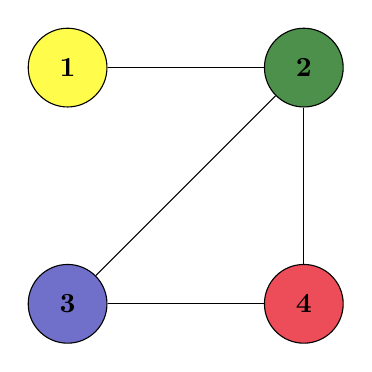
\begin{tikzpicture}[x=1.5cm, y=1.5cm]
  % 設定
  \tikzset{node/.style={circle,draw=black,minimum size=1cm}}
 
  %色
  \definecolor{red}{RGB}{230,0,18}
  \definecolor{blue}{RGB}{51,51,179}
  \definecolor{yellow}{RGB}{255,251,0}
  \definecolor{green}{RGB}{0,96,0}
 
  % 補助線
  % \draw [help lines,blue] (0,0) grid (20,6);
 
  % node %
  \node[node, fill=yellow!70] at (-1,1) (node1) {\textbf{1}};
  \node[node, fill=green!70] at (1,1) (node2) {\textbf{2}};
  \node[node, fill=blue!70] at (-1,-1) (node3) {\textbf{3}};
  \node[node, fill=red!70] at (1,-1) (node4) {\textbf{4}};
 
  \foreach \u / \v in {node1/node2, node2/node3, node2/node4, node3/node4}
  \draw (\u) -- (\v);
\end{tikzpicture}
} &
    \rz{\Large$\Leftarrow$} &
    \scalebox{0.5}{\input{gcrp_t2}}\\
    ゴール状態 ($t=3$) && $t=2$
  \end{tabular}
\end{center}
\end{frame}
%%%%%%%%%%%%%%%%%%%%%%%%%%%%%%%%%%%%%%%%%%%%%%%%%%%%%%%%%%%%%%%%%%%
\begin{frame}\frametitle{$k$彩色遷移問題の性質}

  \begin{itemize}
    \item 色数$k$によって問題の性質が異なることが知られている.
    \begin{itemize}
      \item \structure{$k=2$}のとき,グラフGは2部グラフであり\structure{明らかに到達不能}~[Cereceda+ '08].
      \item \structure{$k=3$}のとき,\structure{クラスP}に属する~[Cereceda+ '08].
      \item \structure{$k \ge 4$}のとき,一般に\structure{\textbf{PSPACE完全}}となる~[Bonsma+ '09].
    \end{itemize}

    \item グラフの形に制限を加えることにより,多項式時間で解決可能となるものが存在することがわかっている~[Bonsma+ '09].
    \begin{itemize}
      \item 平面グラフであり,かつ$k \ge 7$のとき.
      \item 2部平面グラフであり,かつ$k \ge 5$のとき.
    \end{itemize}

  \end{itemize}
\end{frame}

%%%%%%%%%%%%%%%%%%%%%%%%%%%%%%%%%%%%%%%%%%%%%%%%%%
%% 実験結果
%%%%%%%%%%%%%%%%%%%%%%%%%%%%%%%%%%%%%%%%%%%%%%%%%%
%\begin{frame}\frametitle{実験結果: 考察}
%
%  \begin{itemize}
%    \item \code{unchanged}符号化は,\code{changed}符号化と比べて有効性を示した.
%    \item 要因として,\alert{基礎化後のルール数の差}が考えられる.
%    \begin{itemize}
%      \item \textit{clingo}では与えられた論理プログラムを充足可能性判定問題へと変換して解く.
%      \item ルール数を少なくすることは,節数を少なくすることにつながる.
%      \item 節数が多い時,単位伝播やヒューリスティックによる変数選択時のオーバーヘッドが増加する.
%      \item ルール数を抑えることでオーバーヘッドの減少につながり,優位性を示したと考えられる.
%    \end{itemize}
%  \end{itemize}
%  
%\end{frame}

%%%%%%%%%%%%%%%%%%%%%%%%%%%%%%%%%%%%%%%%%%%%%%%%%%
%% 基礎化
%%%%%%%%%%%%%%%%%%%%%%%%%%%%%%%%%%%%%%%%%%%%%%%%%%
%\begin{frame}\frametitle{基礎化}
%  
%\end{frame}

%%%%%%%%%%%%%%%%%%%%%%%%%%%%%%%%%%%%%%%%%%%%%%%%%%
%% ASP符号化のルール数
%%%%%%%%%%%%%%%%%%%%%%%%%%%%%%%%%%%%%%%%%%%%%%%%%%
%\begin{frame}\frametitle{2つの符号化の基礎化後のルール数}
%
%  \begin{itemize}
%    \item 基礎化とは,変数を含む述語論理を変数を含まない命題論理へと変換することである.
%    \item 遷移制約に関するルール数のみに着目する.
%    \item $|L|$をステップ長$\ell$,$|C|$を色数,$|V|$をグラフ$G$の頂点数とする.
%  \end{itemize}
%
%  \begin{exampleblock}{}
%    \centering
%    \begin{tabular}{|c|c|}\hline
  符号化名 & ルール数 \\ \hline
  vrc1 & $4|T|{|C|\choose 2}^{2}{|V|\choose 2}$ \\ \hline
  vrc2 & $|T|\left(2{|C|\choose 2}|V| + 1\right)$ \\ \hline
  vrc3 & $|T|(|CV| + 1)$ \\ \hline
\end{tabular}
%  \end{exampleblock}
%
%  \begin{itemize}
%    \item 遷移制約の基礎化後のルール数は,遷移回数の選び方の組合せ・
%          色の選び方の組合せ・グラフの頂点の選び方の組合せの乗算となる.
%  \end{itemize}
%
%\end{frame}

%%%%%%%%%%%%%%%%%%%%%%%%%%%%%%%%%%%%%%%%%%%%%%%%%%
%% PSPACE
%%%%%%%%%%%%%%%%%%%%%%%%%%%%%%%%%%%%%%%%%%%%%%%%%%
%\begin{frame}\frametitle{クラスPSPACE}
%
%  \begin{itemize}
%    \item 計算量のクラスの一つ.
%    \item 決定性チューリングマシンに多項式量のメモリを与えることで解決できる問題が属する.
%    \item 指数時間で解くことが可能.
%    \item P$\subseteq$NP$\subseteq$PSPACEであることはわかっている.
%    \begin{itemize}
%      \item ただし, 真に包含するかは未解決.
%    \end{itemize}
%  \end{itemize}
%  
%\end{frame}

\backupend